\chapter{System Overview and Workflow}

This chapter presents the architecture and operational workflow of the proposed zero-knowledge proof-based verification system. Through a series of diagrams, we illustrate the theoretical foundation, core processes, and end-to-end architecture that enable privacy-preserving model prediction and accuracy verification.

% ============================================================================
% FIGURE 1: ZKP Process
% ============================================================================
\section{Zero-Knowledge Proof Process}

The ZKP process involves four core stages: \textit{Setup}, where cryptographic parameters are initialized; \textit{Commit}, where inputs and witnesses are securely bound; \textit{Prove}, where the prover generates a succinct proof of correct computation; and \textit{Verify}, where the verifier checks validity using public inputs. This process ensures correctness, soundness, and zero-knowledge without exposing internal data or parameters.

\begin{figure}[H]
\centering
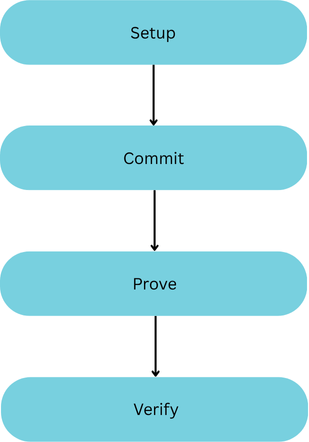
\includegraphics[width=0.4\textwidth]{BTP_ZKP Process.png}
\caption{Zero-Knowledge Proof Process}
\label{fig:zkp_process}
\end{figure}

\clearpage

% ============================================================================
% FIGURE 2: Theoretical Implementation
% ============================================================================
\section{Theoretical Implementation}

This implementation secures a pretrained logistic regression model by keeping its parameters $(w, b)$ confidential. When client inputs are provided as public data, the model generates predictions using the private parameters, and a zero-knowledge proof verifies the correctness of these predictions without revealing the weights or biases. Thus, clients can confirm that predictions are computed correctly using the claimed model while the model parameters remain fully private.

\begin{figure}[H]
\centering
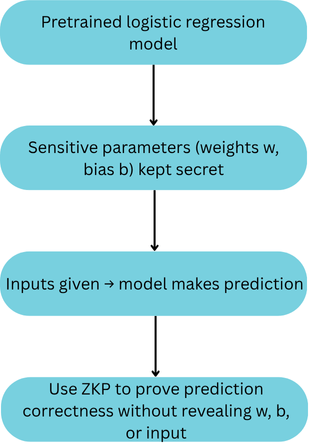
\includegraphics[width=0.4\textwidth]{BTP_Theoretical Implementation.png}
\caption{Theoretical Implementation of Zero-Knowledge Proof System}
\label{fig:theoretical_implementation}
\end{figure}

% ============================================================================
% FIGURE 3: Accuracy Verification Process
% ============================================================================
\section{Accuracy Proof Generation Process}

The Accuracy Proof Generation process begins with two inputs — the model’s claimed accuracy ($A_m$) and the client’s private dataset. The model is executed locally to compute the actual accuracy ($A_c$), and both values are compared inside an arithmetic circuit. If $A_m < A_c$, the system proceeds to generate a succinct SNARK proof certifying that the model’s accuracy claim is correct. The client then verifies this proof without accessing any private data, ensuring honest reporting and privacy-preserving evaluation.

\begin{figure}[H]
\centering
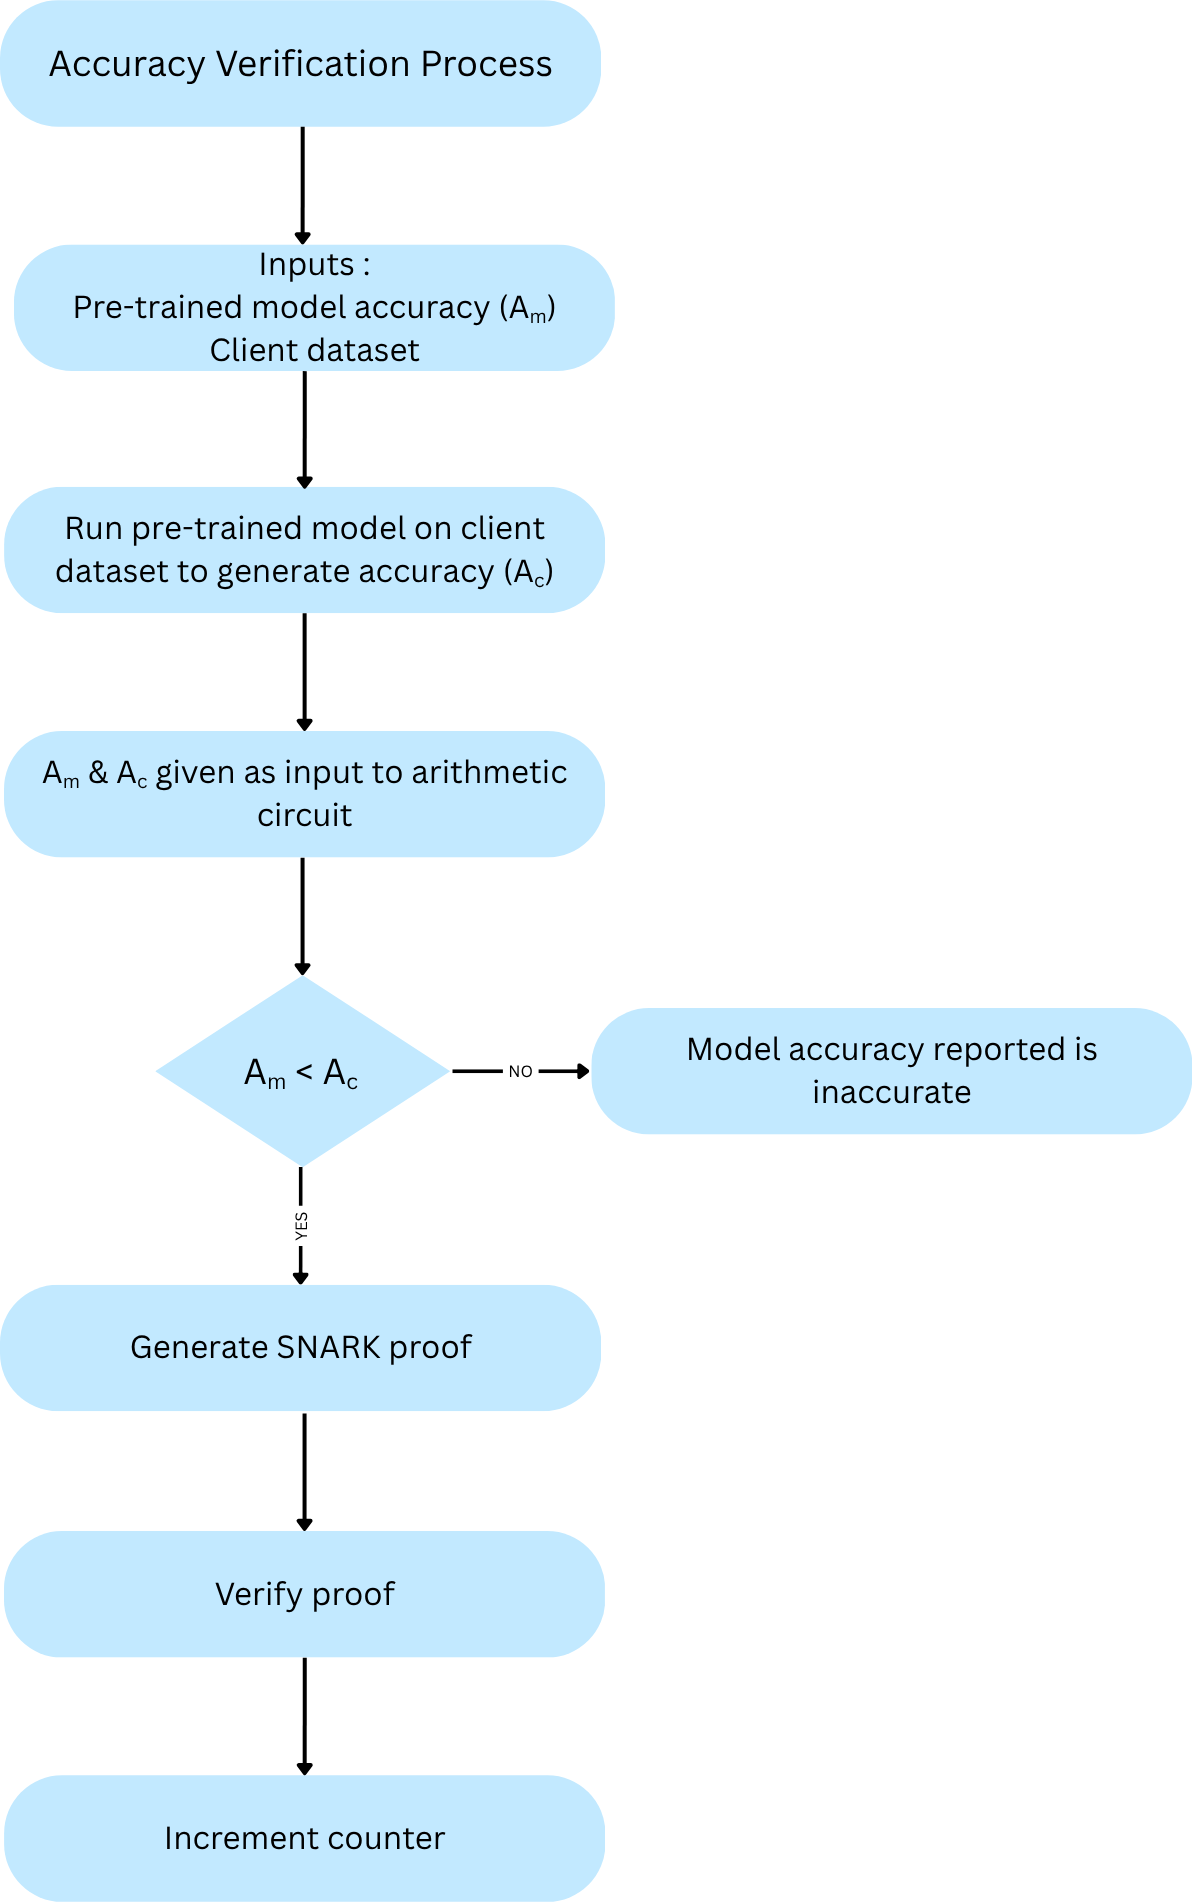
\includegraphics[width=0.6\textwidth]{BTP_Accuracy Proof Process.png}
\caption{Accuracy Verification Process}
\label{fig:accuracy_verification}
\end{figure}

% ============================================================================
% FIGURE 4: System Architecture
% ============================================================================
\section{System Architecture}

The architecture involves three entities: the Client (Verifier), Server (Prover), and a Trusted Third Party responsible for one-time setup. The system operates through a two-layer recursive SNARK framework. In the first layer, the server generates batch proofs for groups of samples, where each batch proof cryptographically verifies the correctness of individual predictions and counts the number of accurate predictions within that batch. In the second layer, an aggregator circuit recursively composes these batch proofs to verify that the total accuracy across all batches meets or exceeds the claimed threshold. The client receives a single compact final proof $\pi_{final}$ along with public inputs including the dataset hash, total sample count, and aggregate correct prediction count. By verifying this constant-size proof, the client can confirm the model's accuracy claim without learning individual predictions or model parameters, achieving scalable and privacy-preserving prediction and accuracy verification.

\begin{figure}[H]
\centering
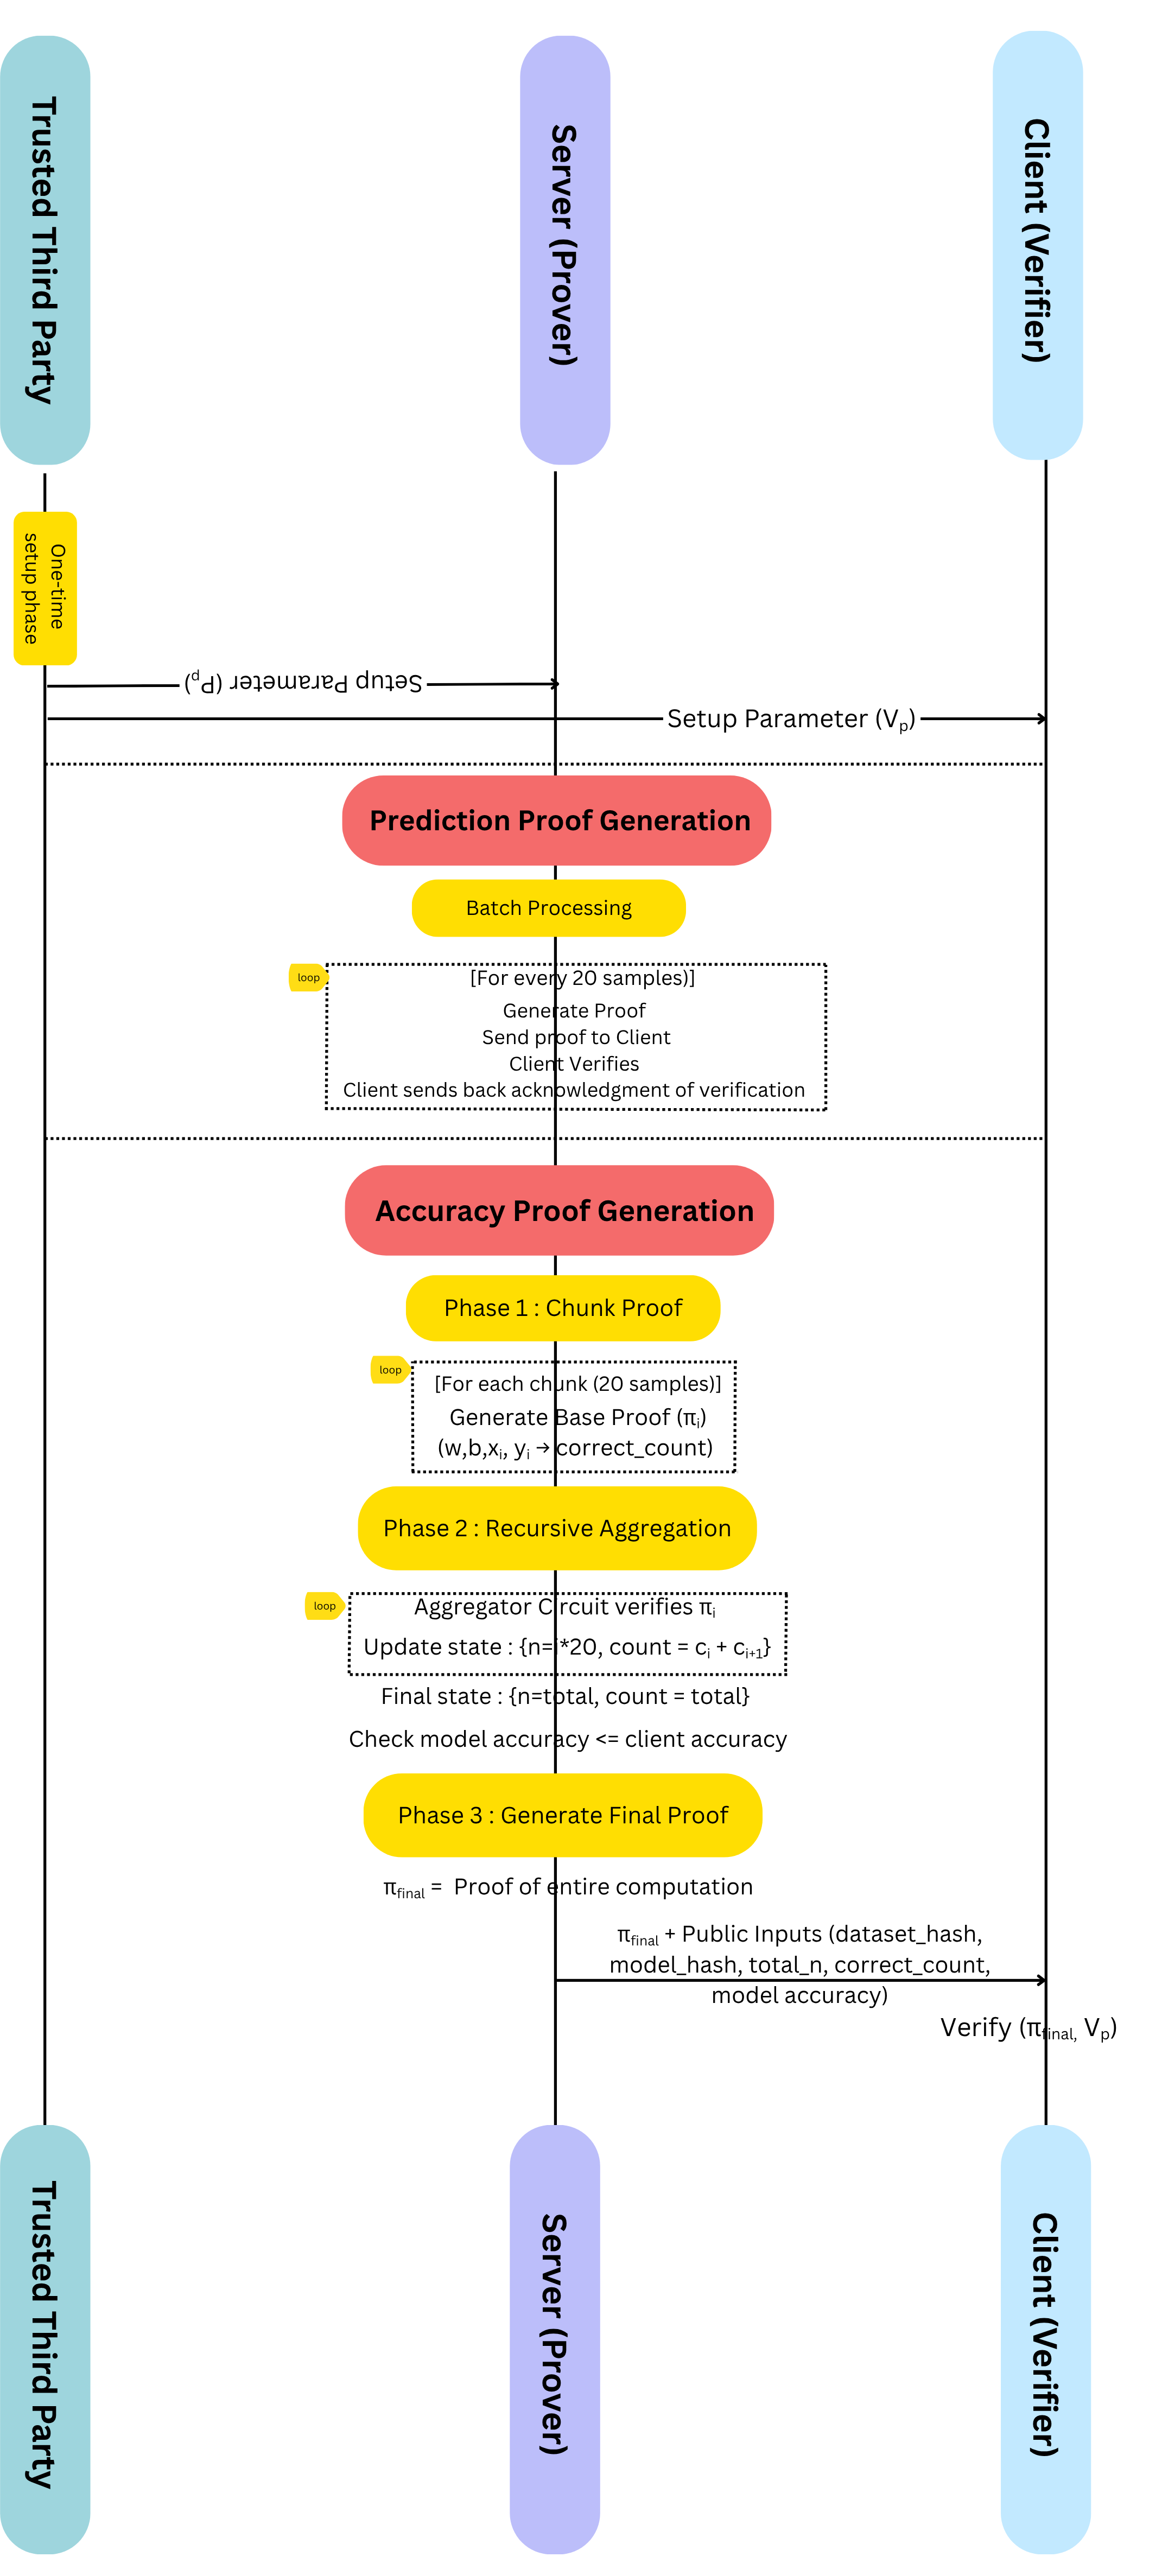
\includegraphics[width=0.565\textwidth]{sysarch.png}
\caption{System Architecture for Prediction Proof and Accuracy Proof generation}
\label{fig:system_architecture}
\end{figure}
